\documentclass[11pt]{article}

\usepackage[T1]{fontenc}
\usepackage[utf8]{inputenc}
\usepackage{lmodern}
\usepackage[margin=2.4cm]{geometry}
\usepackage{amsmath,amssymb}
\usepackage{graphicx}
\usepackage{booktabs}
\usepackage{tabularx}
\usepackage{array}
\newcolumntype{L}[1]{>{\raggedright\arraybackslash}p{#1}}
\newcolumntype{Y}{>{\raggedright\arraybackslash}X}
\usepackage{multirow}
\usepackage{xcolor}
\usepackage{microtype}
\usepackage{enumitem}
\usepackage{float}
\usepackage[round,sort&compress]{natbib}
\usepackage[hidelinks]{hyperref}
\usepackage{caption}
\captionsetup{font=small,labelfont=bf}
\setlist{itemsep=2pt,topsep=4pt}

\newcommand{\pending}{\textcolor{gray}{--}}
\newcommand{\nb}[1]{\texttt{#1}}

\title{\textbf{Benchmarking next-visit diagnosis prediction for rare labels on MIMIC-IV}\\[4pt]
\large Classic, Transformer, knowledge-based, looped and adaptive-depth models under one protocol}
% Co-authors to be confirmed: P. Li\`o, A. Dussolle, C. d'Ercoli, C. Bernard, A. Popescu.
\author{Timoth\'ee Roina\\
\small Pietro Li\`o group, Department of Computer Science and Technology, University of Cambridge}
\date{November 2026}

\begin{document}
\maketitle

\begin{abstract}
Models that predict the diagnoses of a patient's next hospital admission are much weaker on rare labels than on
frequent ones, and each new method reports its gains under its own preprocessing, label space, frequency groups
and training protocol. Before proposing yet another architecture for rare diseases, we need to know where the
existing ones stand on equal terms. We therefore benchmark 21 models on MIMIC-IV under a single protocol: simple
baselines (label prior, bag of codes), recurrent models (GRU, RETAIN), the Transformer backbone shared by recent
concept encoders and four of its variants (visit positions, attention pooling within visits, cross-modality
attention, logit adjustment), knowledge-based embeddings (GRAM; text embeddings with retrieval of rare-disease
knowledge), deeper Transformers, and looped Transformers with and without adaptive depth. For looped models we
compare, at equal parameters and equal compute, a \emph{layer loop} (each layer repeated before the next) with a
\emph{model loop} (the whole stack repeated). Building the benchmark required three corrections that change the
numbers reported in the literature and in our own earlier work: the code mapping used by our preprocessing and by
MedCo mislabels 10.7\% of ICD-10 diagnosis rows (for instance, essential hypertension becomes a hypertensive
complication), the frequency groups used by MedCo's evaluation are not equal-size quartiles, and only 37\% of the
rare diseases listed in the Mondo ontology can be expressed in the CCS label space at all. [Benchmark results:
to be inserted from the cluster runs; every number in this report is measured, none is projected.]
\end{abstract}

\section{Introduction}

Multi-label next-visit diagnosis prediction takes the coded history of a patient's first $k$ admissions
(diagnoses, procedures and medications) and outputs a probability for every diagnosis label at admission $k+1$.
Because each label is scored separately, the task makes the long tail visible. On MIMIC-IV, the most recent concept
encoders report that the base Transformer reaches 46.80 AUPRC on their least frequent label group against 77.20 on
the most frequent one; LINKO \citep{linko2025} raises the former to 49.61 and MedCo \citep{medco2026} to 52.01, but
the difference between the two groups only moves from 30.40 to 29.18 points \citep[Table 1]{medco2026}.

These comparisons are made within each paper. Across papers, the cohorts, the code mappings, the label spaces,
the definition of frequency groups and the training budgets differ, and several of these choices interact with
rarity: a different mapping changes which labels are rare, a different grouping changes what ``rare'' means in
the metric. Meanwhile, model families that have not been evaluated on this task at all have appeared, in
particular looped Transformers that reuse their layers to add computation without parameters
\citep{dehghani2019universal,giannou2023looped,yang2024looped,geiping2025recurrent,zhu2025ouro} and can adapt their
depth to the input \citep{graves2016act,banino2021pondernet,popescu2026adaptive}. Rare labels are a natural place
to test whether extra, input-dependent computation helps.

Our position is simple: to improve rare-disease prediction we first need a benchmark in which every model is
trained and evaluated in the same way, with the rare-label metrics stated precisely. This report describes such a
benchmark (Sections~\ref{sec:design} and~\ref{sec:models}), its results (Section~\ref{sec:results}), and what a
``rare'' label means in it (Section~\ref{sec:rare}).

\section{Benchmark design}\label{sec:design}

\subsection{Cohort and codes}
\paragraph{Cohort.} We use the \texttt{hosp} module of MIMIC-IV \citep{johnson2023mimiciv}. Adult patients
with at least two admissions are kept (100,163 patients), and patients are split 70/15/15 into training,
validation and test sets (70,114 / 15,024 / 15,025 patients). For training, every history length
$k \in \{1,\dots,K-1\}$ of a patient with $K$ admissions gives one sample; validation and test patients give one
sample each, with $k=\lfloor K/2\rfloor$. This yields 225,024 / 15,004 / 15,010 samples.

\paragraph{Codes.} ICD-10 codes (54.3\% of diagnosis rows) are converted to ICD-9 with the CMS General
Equivalence Mappings \citep{cms2018gem}, keeping the first target listed, and ICD-9 diagnoses are mapped to the
most specific level of the HCUP multi-level CCS \citep{hcup2015}. Procedures are mapped to CCS procedure
categories and prescriptions (NDC) to ATC level~3, both through PyHealth \citep{yang2023pyhealth}. The input
vocabularies contain 576 diagnosis, 230 procedure and 201 medication codes. An average admission carries
11.7 diagnosis, 1.6 procedure and 18.1 medication codes.

\paragraph{Codes.} ICD-10 codes (54.3\% of diagnosis rows) are converted to ICD-9 with the CMS General
Equivalence Mappings \citep{cms2018gem} and ICD-9 diagnoses are mapped to the most specific level of the HCUP
multi-level CCS \citep{hcup2015}. Procedures are mapped to CCS procedure categories and prescriptions (NDC) to ATC
level~3, both through PyHealth \citep{yang2023pyhealth}. The input vocabularies contain 576 diagnosis, 230
procedure and 201 medication codes; an average admission carries 11.7 diagnosis, 1.6 procedure and 18.1
medication codes.

\subsection{Labels and their correction}\label{sec:labelfix}

The labels are the CCS categories of all diagnoses of admission $k+1$, including those already present in the
history, as in MedCo \citep{medco2026}. The original preprocessing, like MedCo's released code, keeps the first
ICD-9 target that the GEM lists for each ICD-10 code. The GEM lists several targets for 7,862 ICD-10-CM codes, and
for 3,864 of them the targets fall into different CCS categories: 3,572 are combination entries (one ICD-10 code
corresponds to two ICD-9 codes, and keeping the first drops one) and 292 are lists of alternatives, where the
first one is an arbitrary choice.

\paragraph{Extent of the artefact.} 368,210 ICD-10 diagnosis rows (10.7\%) carry a code whose GEM targets fall
into more than one CCS category. \texttt{I10} alone accounts for 83,775 rows and 48,611 patients. Under the
original rule, ``Essential hypertension'' (7.1.1) is reached by 53,401 patients through ICD-9 rows and by only
1,915 through ICD-10 rows, whereas ``Other hypertensive complications'' (7.1.2.2) is reached by 543 patients
through ICD-9 rows and by 48,727 through ICD-10 rows; in the ICD-9 era, malignant essential hypertension (401.0),
the target chosen for \texttt{I10}, is coded in only 397 rows. We corrected the mapping by sending combination
entries to the union of their targets and resolving lists of alternatives with the target most often coded in
the ICD-9 era. Among patients with at least two admissions, the correction changes the patient count of 30 of
576 labels by 25\% or more (Table~\ref{tab:gemfix}). Three examples show how arbitrary the first target can be:
bacteraemia (\texttt{R78.81}) is sent to \emph{bacteraemia of newborn}, so the label ``Other perinatal
conditions'' is given to 1,957 adult patients; toxic encephalopathy (\texttt{G92}) is sent to toxic
encephalitis; acute respiratory failure with hypoxia (\texttt{J96.01}) is sent to respiratory failure following
trauma or surgery.

\begin{table}[H]
\centering\small
\begin{tabular}{llrr}
\toprule
CCS & label & original rule & corrected\\
\midrule
7.1.1 & Essential hypertension & 34,621 & 51,965\\
7.1.2.2 & Other hypertensive complications & 29,159 & 582\\
7.2.11 & Congestive heart failure; nonhypertensive & 9,826 & 19,433\\
8.6.1 & Respiratory failure & 5,723 & 13,712\\
8.6.2 & Other respiratory insufficiency & 11,089 & 3,094\\
6.1.2 & Encephalitis (except that caused by TB or STD) & 4,777 & 359\\
15.7 & Other perinatal conditions & 1,957 & 1\\
\bottomrule
\end{tabular}
\caption{Patients (with at least two admissions) carrying selected labels under the original mapping and under
the corrected mapping (Notebook 9).}
\label{tab:gemfix}
\end{table}


The benchmark therefore uses the corrected labels (\texttt{scripts/relabel\_gem.py}): cohort, visits, splits,
history lengths, procedures and medications are unchanged, and only the diagnosis inputs and targets are
recomputed, after which the label vocabulary and frequency strata are rebuilt with the original procedure. The
MedCo backbone is also trained on the original labels to measure the effect of the correction.

\subsection{Metrics and frequency groups}
We report two kinds of AUPRC, which behave very differently on rare
labels. \emph{Sample-AUPRC} (the PyHealth and MedCo convention) computes the average precision within each test
sample over the labels and averages over samples; restricted to a group of labels, it keeps the samples with at
least one positive in that group. \emph{Label-AUPRC} computes the average precision of each label over test
samples and averages over labels. Frequency groups are defined on training data only. Our main analysis uses
four groups of 143 labels each, split at the quartiles of the number of training samples containing the label
($Q_{25}=200$, $Q_{50}=1{,}132$, $Q_{75}=4{,}258$). Notebook~1 stores a second, patient-level split
($Q_{25}=166$) used for the ``rare/medium/common'' strata. The grouping used in MedCo's evaluation code is a
third definition, discussed below.


\paragraph{Frequency groups in MedCo.} In our first run of the backbone under the original protocol
(Table~\ref{tab:nb2}), the least frequent group scored far lower than the least frequent group reported by MedCo for
the same backbone (0.290 against 0.468). Reading their
evaluation code (\nb{utils/eval\_test.py}, function \nb{get\_group\_labels1}) explains most of the
discrepancy. Labels are sorted by frequency and assigned to the group in which the \emph{cumulative share of
label occurrences} falls, so each group holds a quarter of the occurrences rather than a quarter of the
labels. With a label distribution as skewed as ours (the 20 most frequent labels account for 28.5\% of
label occurrences, counted per training patient), the first group contains most of the vocabulary and the last only a handful of very frequent
labels. The columns of each group are selected by the insertion order of a \texttt{Counter}, which matches the label indices only if the label tokenizer happens to use the same
order; we have not run their code to check this. The published group-wise numbers are therefore not comparable
with ours, and our earlier reading of their ``0--25\%'' group as the rarest quarter of labels was wrong.
The benchmark reports both definitions for every model.


\subsection{Training protocol}

All models are trained with binary cross-entropy (or the model's own objective for adaptive depth and logit
adjustment), Adam with learning rate $10^{-3}$, batch size 64, gradient clipping at 1.0, at most 50 epochs and early
stopping on validation sample-AUPRC with patience 5, on one 10\,GB slice of an NVIDIA A100. Embedding dimension
is 256 and dropout 0.5 throughout. Each configuration is run with three seeds (42, 123, 7); we report means and
standard deviations, and differences on the rarest quartile are tested with a paired bootstrap over test samples.
About 700 test samples have a positive in the rarest quartile, so differences below one point are within noise.

\section{Models}\label{sec:models}

\begin{table}[H]
\centering\footnotesize
\begin{tabular}{lllr}
\toprule
family & model & description & block appl.\\
\midrule
baseline & \texttt{label\_prior} & training label frequencies & 0\\
 & \texttt{bag\_of\_codes} & code counts of the history + MLP & 0\\
\midrule
recurrent & \texttt{gru} & GRU over sum-pooled visits & 0\\
 & \texttt{retain} & RETAIN & 0\\
\midrule
transformer & \texttt{transformer} & MedCo backbone (1 layer per modality, concat) & 1\\
 & \texttt{transformer\_pos\_last} & + visit positions, last-visit readout & 1\\
 & \texttt{transformer\_setpool} & + attention pooling within visits & 1\\
 & \texttt{transformer\_cross} & + cross-modality attention & 1\\
 & \texttt{transformer\_logitadj} & + logit-adjusted loss & 1\\
\midrule
knowledge & \texttt{gram} & GRAM ontology embeddings (CCS, ATC) & 1\\
 & \texttt{knowledge\_rag\_readout} & RAG-initialised embeddings + knowledge readout & 1\\
\midrule
deep & \texttt{deep\_L2} & 2 distinct layers & 2\\
 & \texttt{deep\_L4} & 4 distinct layers & 4\\
\midrule
looped & \texttt{loop\_T4} & 1 layer applied 4 times & 4\\
 & \texttt{layerloop\_L2T2} & layer loop: L1 L1 L2 L2 & 4\\
 & \texttt{modelloop\_L2T2} & model loop: L1 L2 L1 L2 & 4\\
\midrule
adaptive & \texttt{deep\_L4\_adaptive} & 4 distinct layers, exit after any layer & 4\\
 & \texttt{loop\_T4\_adaptive} & loop T4, geometric depth prior, post-hoc exit & 4\\
 & \texttt{loop\_T4\_gate} & loop T4, PonderNet gate & 4\\
 & \texttt{layerloop\_L2T2\_adaptive} & layer loop, geometric depth prior, post-hoc exit & 4\\
 & \texttt{modelloop\_L2T2\_adaptive} & model loop, geometric depth prior, post-hoc exit & 4\\
\bottomrule
\end{tabular}

\caption{The 21 models of the benchmark. ``Block appl.'': number of Transformer block applications per modality
(the compute of the Transformer part, at equal width).}
\label{tab:models}
\end{table}

\paragraph{Baselines and recurrent models.} The label prior predicts the training frequency of each label and gives
the floor of every metric. The bag-of-codes model feeds the logarithm of the count of each code in the history to
a one-hidden-layer MLP; because targets include recurrent diagnoses, this model can copy the history and is a
stronger baseline than its simplicity suggests. The GRU encodes the sequence of visit vectors (sum of code
embeddings of each modality, concatenated), as in Doctor AI; RETAIN adds two reverse-time attention mechanisms over
visits and variables \citep{choi2016retain}.

\paragraph{Transformer backbone and variants.}
The model follows the released MedCo code \citep{medco2026}. Each modality has its own
embedding matrix ($d=256$, initialised from $\mathcal N(0,0.01^2)$); the codes of a visit are summed; three
independent single-layer, single-head PyHealth Transformers encode the three visit sequences; their outputs are
concatenated and a linear layer with a sigmoid gives the 572 probabilities. Training minimises binary
cross-entropy with Adam (learning rate $10^{-3}$, batch size 64, dropout 0.5), with early stopping on validation
sample-AUPRC. Two details of the PyHealth layer, shared with MedCo, are worth stating because they are easy to
misread. The patient representation is the output at the \emph{first} visit position (\texttt{x[:, 0, :]}),
not at the last visit; and the layer adds no positional encoding, so attention is bidirectional and blind to
the order of visits beyond the identity of the first one. The model therefore cannot use recency, which is a
limitation for a next-visit task and an obvious ablation for later work.


Four variants change one element each: learned embeddings of the distance to the last visit with a readout at the
last visit (\texttt{transformer\_pos\_last}); attention pooling over the codes of a visit, one Set Transformer block
followed by pooling with a learned seed \citep{lee2019settransformer} (\texttt{transformer\_setpool}); one
cross-modality attention layer over the visit states of the three modalities (\texttt{transformer\_cross}), since in
the backbone modalities meet only in the final linear layer; and logit adjustment
\citep{menon2021logit}, which adds the log prior odds of each label to its logit during training only
(\texttt{transformer\_logitadj}).

\paragraph{Knowledge-based embeddings.} GRAM \citep{choi2017gram} builds each diagnosis and medication embedding by
attention over the code and its ancestors (CCS levels, ATC levels). The knowledge model initialises every code
embedding from a frozen biomedical sentence encoder, BioLORD-2023 \citep{remy2024biolord}, as
$z_i = a\,W e_i + \delta_i$ with a learned projection $W$ and a free correction $\delta_i$. For diagnosis
categories the encoded text is augmented with knowledge retrieved from Mondo and the HPO annotations: the diseases
whose ICD-10-CM cross-references map to the category (rare diseases first), their most frequent phenotypes and
genes (Section~\ref{sec:rare}). The same label documents also enter the classifier, $\ell_r=(w_r+Ue_r)^\top h$
with $U$ shared by all labels, so that a rare label can inherit a direction learned on frequent labels with
similar descriptions \citep{rios2018fewshot}. This combines the ideas of concept encoders that enrich embeddings
from ontologies and LLMs \citep{linko2025,medco2026,jiang2024graphcare,hegselmann2025} with retrieval
augmentation \citep{xu2024ramehr,jiang2025kare}.

\subsection{Depth: deep, looped and adaptive Transformers}

Per modality, a stack holds $L$ distinct Transformer blocks applied along a schedule of $D$ block indices. A deep
Transformer uses distinct blocks, schedule $(1,2,\dots,D)$. A looped Transformer reuses blocks: \texttt{loop\_T4}
applies a single block four times, $(1,1,1,1)$. With two blocks and four applications there are two ways to loop:
\begin{itemize}
\item \textbf{layer loop}, $(1,1,2,2)$: each layer is iterated before passing to the next, so the representation
is refined at one level of abstraction before moving on;
\item \textbf{model loop}, $(1,2,1,2)$: the whole stack is iterated, as in Universal-Transformer-style and
recurrent-depth models \citep{dehghani2019universal,geiping2025recurrent}, so that later iterations can revisit
early processing in the light of later layers.
\end{itemize}
\texttt{deep\_L4}, \texttt{loop\_T4}, \texttt{layerloop\_L2T2} and \texttt{modelloop\_L2T2} have the same compute
(four block applications); the looped ones have the parameters of one or two blocks, and \texttt{deep\_L2} has the
parameters of the two-block loops with half their compute. This separates the effect of computation from that of
parameters.

\paragraph{Adaptive depth.} The adaptive versions are read out after every block application with the shared
classifier and trained on all exits, weighted by a truncated geometric prior over depths ($\lambda=0.3$), or with a
PonderNet halting distribution \citep{banino2021pondernet} (\texttt{loop\_T4\_gate}); all adaptive models,
including the gated one, are evaluated with the same post-hoc exit rules. At test time, following
\citet{popescu2026adaptive}, who found that post-hoc confidence readouts match or beat learned halting gates, each
sample exits at the first depth where the mean binary entropy of its top-$m$ predicted labels (or the change since
the previous depth) falls below a threshold. The threshold is chosen on validation as the most aggressive one that
keeps 99\% of the full-depth validation sample-AUPRC. We report the resulting accuracy, the average exit depth, and
the average exit depth of samples with a rarest-quartile target against the others: if rare labels need more
computation, their samples should exit later. \texttt{deep\_L4\_adaptive} applies the same procedure to a
non-looped stack.

\paragraph{A pitfall of weight tying.} The first cluster runs degraded with depth: after two epochs the gated
model scored 0.463 at depth 1 and 0.436 at depth 4 (validation sample-AUPRC), the model trained on the last
iteration only reached 0.382 after three epochs, against 0.447 for a single pass after one, and the model
trained with a uniform prior collapsed at depths 3 and 4 (0.367 $\rightarrow$ 0.239 between epochs 1 and 2).
The cause is in the PyHealth block, which ends with \texttt{return self.dropout(x)}: a dropout of rate 0.5 applied
to its whole output, residual stream included. In a single pass this is harmless; in a loop it hits the
recurrent state at every iteration, so after four iterations a coordinate of the input survives on the direct
path with probability $0.5^4=1/16$ during training. We moved this dropout from the recurrent path to the
readout branch. For $T=1$ the training distribution is unchanged (the same two dropouts precede the readout),
and in evaluation mode the two versions are identical for every $T$. All multi-block models of the benchmark, looped or not, use this fix, so that they
differ only in their schedule. A one-epoch run of the single-pass configuration on a 10\,GB slice of an A100
reproduced the Notebook 2 model exactly (identical logits) and took 10.6 minutes per epoch; four-block
configurations took 12 to 14 minutes per epoch.


\section{Results}\label{sec:results}

\subsection{Reference run under the original protocol}

Before the benchmark, the backbone was trained once on the original labels, on a laptop, and stopped by hand
after seven epochs; the best validation sample-AUPRC was reached at epoch 5 (0.4723). Table~\ref{tab:nb2} gives its
test results. The validation macro label-AUPRC was still rising at epoch 7 (Figure~\ref{fig:nb2}), which means that
early stopping on sample-AUPRC, chosen for comparability with MedCo, selects a model that has not finished learning
the infrequent labels; the benchmark keeps this criterion for comparability but also records the per-label
metrics at every epoch.

\begin{table}[H]
\centering\small
\begin{tabular}{lccccc}
\toprule
 & all labels & Q1 (rarest) & Q2 & Q3 & Q4 (most frequent)\\
\midrule
labels in group & 572 & 143 & 143 & 143 & 143 \\
test samples with $\ge 1$ positive in group & 15,010 & 702 & 4,915 & 10,667 & 14,812\\
test sample-AUPRC & 0.4707 & 0.2896 & 0.3052 & 0.3674 & 0.5429\\
\bottomrule
\end{tabular}
\caption{Backbone (Notebook 2), best validation epoch, test set. Groups are equal-size quartiles of the
number of training samples containing each label. The Q4$-$Q1 gap is 0.253.}
\label{tab:nb2}
\end{table}

\begin{figure}[H]
\centering
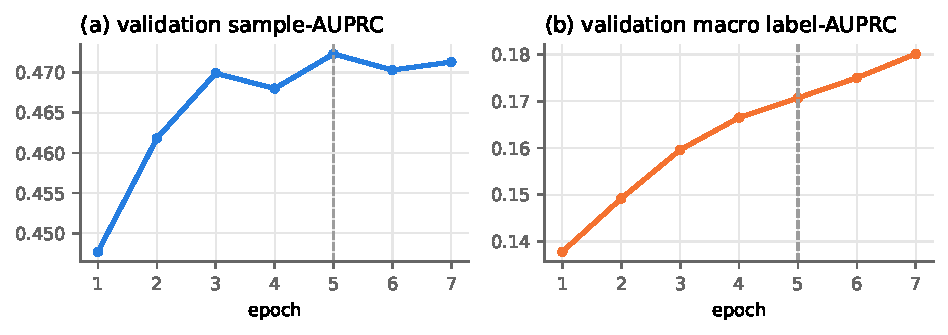
\includegraphics[width=0.8\linewidth]{figures/nb2_validation_curves.pdf}
\caption{Validation curves of the backbone. The dashed line marks the epoch selected by early stopping on
sample-AUPRC. Training was interrupted after epoch 7.}
\label{fig:nb2}
\end{figure}



\subsection{Benchmark}

\IfFileExists{tables/benchmark_main.tex}{%
\begin{table}[H]
\centering\scriptsize
\resizebox{\linewidth}{!}{\input{tables/benchmark_main.tex}}
\caption{Test results on the corrected labels, mean (and standard deviation) over seeds. ``all'', Q1--Q4:
sample-AUPRC overall and restricted to each equal-size label-frequency quartile; ``label Q1'', ``label Q4'': macro
label-AUPRC of the rarest and most frequent quartiles.}
\label{tab:bench}
\end{table}

\begin{figure}[H]
\centering
\includegraphics[width=0.7\linewidth]{figures/benchmark_overall_vs_q1.pdf}
\caption{Overall vs rarest-quartile sample-AUPRC of every model.}
\label{fig:scatter}
\end{figure}
}{%
\begin{center}
\fbox{\parbox{0.9\linewidth}{\small\textbf{Pending.} The benchmark runs on the HubIA DGX
(\texttt{scripts/benchmark.sbatch}, Notebook 10). Notebook 10 writes \texttt{report/tables/benchmark\_main.tex}
and \texttt{benchmark\_depth.tex}; recompiling this document inserts the tables and figures here.}}
\end{center}
}

\subsection{Depth, looping and adaptive exit}

\IfFileExists{tables/benchmark_depth.tex}{%
\begin{table}[H]
\centering\scriptsize
\resizebox{\linewidth}{!}{\input{tables/benchmark_depth.tex}}
\caption{Deep, looped and adaptive models. ``appl.'': block applications per modality. ``adaptive'': accuracy with
the post-hoc entropy exit chosen on validation; ``mean exit'': average number of block applications used, for
samples with a rarest-quartile target and for the others.}
\label{tab:depth}
\end{table}
\IfFileExists{figures/benchmark_depth_curves.pdf}{%
\begin{figure}[H]
\centering
\includegraphics[width=0.85\linewidth]{figures/benchmark_depth_curves.pdf}
\caption{Test sample-AUPRC when every sample exits after a fixed number of block applications.}
\end{figure}}{}
}{\begin{center}\fbox{\parbox{0.9\linewidth}{\small\textbf{Pending} (same runs).}}\end{center}}

The questions this section answers are: whether four block applications beat one at equal parameters (\texttt{loop\_T4}
against \texttt{transformer}) and at equal compute (\texttt{loop\_T4} against \texttt{deep\_L4}); whether layer loop or
model loop is the better way to reuse two blocks; whether gains, if any, concentrate on the rarest quartile; and
whether adaptive exit saves computation, and spends more of it on samples with rare targets.

\section{What ``rare'' means in this benchmark}\label{sec:rare}

The labels are CCS categories, designed for health-services research. A rare disease in the usual sense
(prevalence below 1 in 2,000 in the European definition; an analysis of 6,172 rare diseases in Orphanet estimated
their cumulative point prevalence at 3.5--5.9\% \citep{nguengang2020prevalence}) is a different object. This
section relates the two, first with public resources and then on the MIMIC-IV diagnosis table.

\subsection{Rare diseases in the CCS label space}

We used only public resources here (Notebook 4): the Mondo Disease Ontology
(commit \texttt{d3bdb9d}, 24 November 2026), whose \texttt{rare} subset unifies the rare-disease lists it
integrates and which cross-references ICD-10-CM, Orphanet and OMIM \citep{vasilevsky2026mondo}; the HPO
annotations (release 2025-01-16), which attach phenotypes and genes to OMIM and Orphanet diseases
\citep{gargano2024hpo}; the 2018 GEM file used by our preprocessing; and the 2015 multi-level CCS tables, read
from the data files of the \texttt{icd} R package \citep{wasey_icd}. Our reconstruction of the label mapping
reproduces the preprocessing exactly: 15,072 ICD-9 codes, 589 CCS categories, and identical results on the five
codes checked in Notebook~1.

\paragraph{Coverage.} We use two definitions. The \emph{broad} one is Mondo's \texttt{rare} subset, the union of
the rare-disease lists that Mondo integrates (Orphanet, GARD, NORD, DOID, NCIt); it includes conditions such
as fibromyalgia, listed by NORD, or toxic encephalopathy, listed by GARD. The \emph{strict} one keeps the
diseases that Orphanet itself classifies as rare. Mondo contains 31,828 non-obsolete diseases, 16,370 in the
broad and 6,331 in the strict subset (Table~\ref{tab:coverage}). Under the broad definition, only 1,020 rare diseases (6.2\%) have an ICD-10-CM code marked as equivalent;
6,116 (37.4\%) have any ICD-10-CM cross-reference, most of them broader codes inherited from Orphanet's
alignment. Through the preprocessing pipeline, 6,066 rare diseases (37.1\%) reach at least one CCS category; the
other 63\% cannot be expressed in this label space at all, whatever the model. Orphanet-rare diseases are better
connected to ICD-10 (61.7\% reach a CCS category), but most of these links are broader codes rather than exact
equivalents (8.2\%).

\begin{table}[H]
\centering\small
\begin{tabular}{lrrrr}
\toprule
 & \multicolumn{2}{c}{broad (Mondo \texttt{rare})} & \multicolumn{2}{c}{strict (Orphanet rare)}\\
\cmidrule(lr){2-3}\cmidrule(lr){4-5}
 & diseases & \% & diseases & \%\\
\midrule
diseases in the subset & 16,370 & 100.0 & 6,331 & 100.0\\
with an exact ICD-10-CM cross-reference & 1,020 & 6.2 & 518 & 8.2\\
with any ICD-10-CM cross-reference & 6,116 & 37.4 & 3,937 & 62.2\\
reaching $\ge 1$ CCS category through the preprocessing & 6,066 & 37.1 & 3,908 & 61.7\\
with an Orphanet cross-reference & 8,669 & 53.0 & 6,331 & 100.0\\
with an OMIM cross-reference & 7,830 & 47.8 & 3,203 & 50.6\\
with HPO phenotype annotations & 9,232 & 56.4 & 4,801 & 75.8\\
with a gene association & 6,769 & 41.4 & 2,946 & 46.5\\
\bottomrule
\end{tabular}
\caption{Rare diseases in Mondo (31,828 non-obsolete diseases in total) and their links to the label space and
to phenotype and gene knowledge, under two definitions (Notebook 4).}
\label{tab:coverage}
\end{table}

\paragraph{Concentration.} The 6,066 reachable rare diseases fall into 274 of the 589 CCS categories, with a
median of 6 rare diseases per hosting category (interquartile range 2--18) and a very long tail
(Figure~\ref{fig:rare}); under the strict definition, 3,908 diseases fall into 250 categories
(median 4). The ten largest categories receive 49.4\% of all disease--category links. They are
residual categories: ``All other congenital anomalies'' (1,076 rare diseases; 889 under the strict definition), ``Other and unspecified
metabolic, nutritional, and endocrine disorders'' (670), ``Other and unspecified hereditary and degenerative
nervous conditions'' (315), followed by congenital anomalies of the limbs and of the integument. For such a
label, a positive sample can stand for any of hundreds of unrelated conditions, and predicting it means
predicting a mixture. The ICD-10-CM three-character level, our secondary label space, is finer (705 categories
host at least one rare disease, median 3) but has the same structure: Q87, ``other specified congenital
malformation syndromes affecting multiple systems'', alone receives 784 rare diseases.

\begin{figure}[H]
\centering
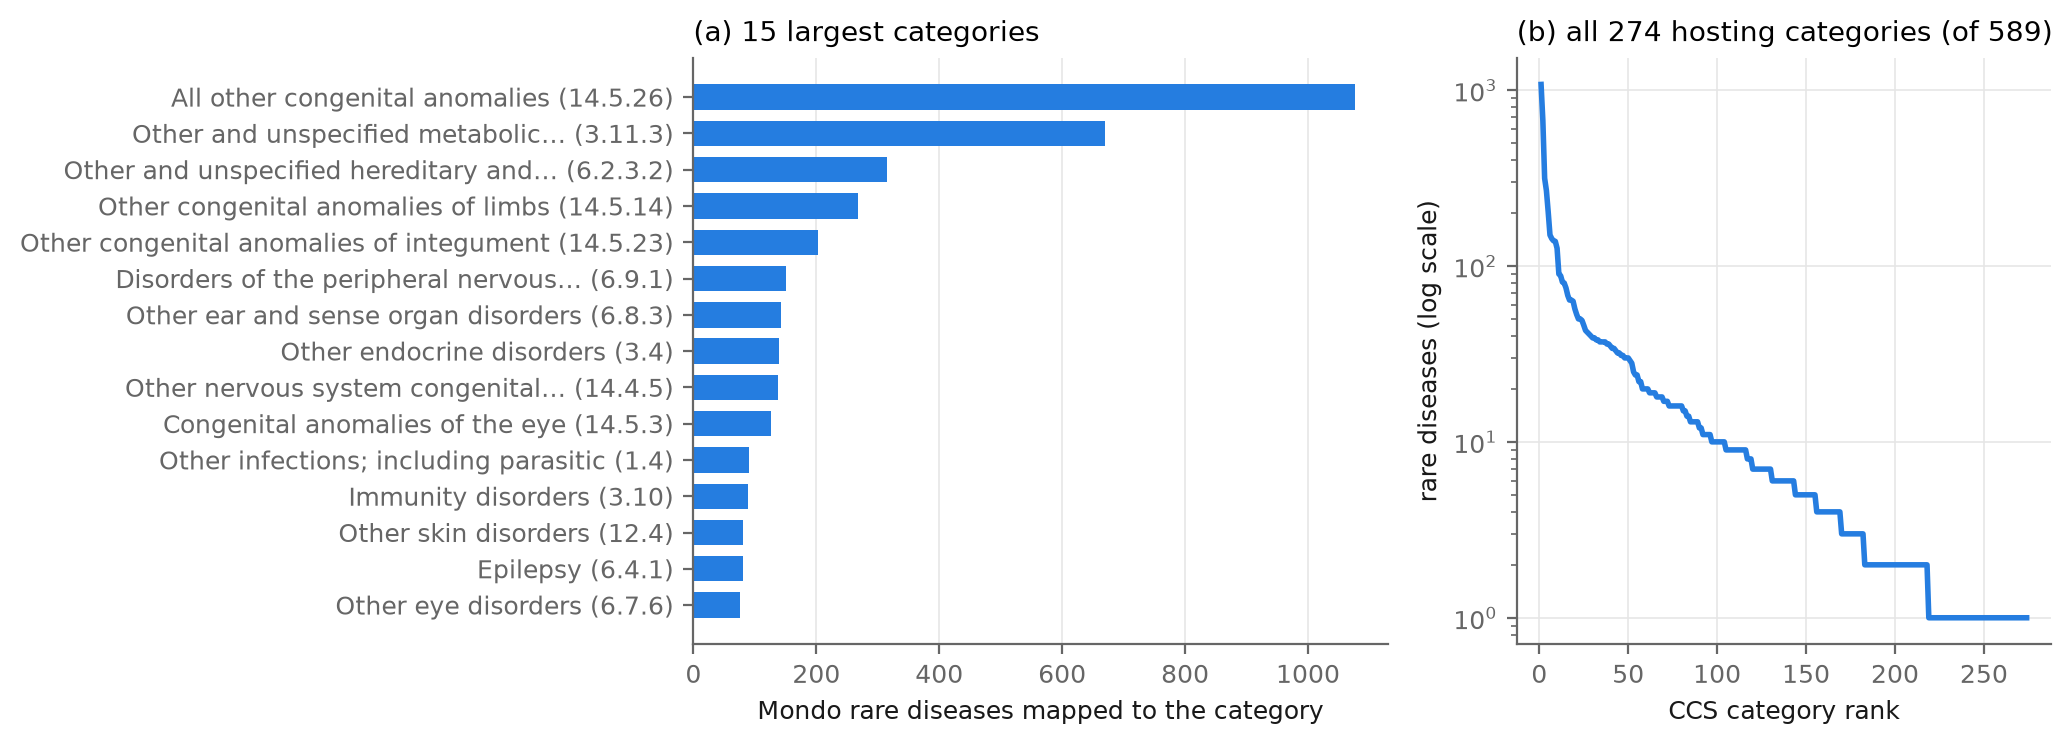
\includegraphics[width=\linewidth]{figures/rare_diseases_per_ccs.png}
\caption{Mondo rare diseases per CCS category, through the preprocessing pipeline (ICD-10-CM
$\rightarrow$ GEM $\rightarrow$ multi-level CCS). (a) The 15 categories with the most rare diseases. (b) All
274 hosting categories, ranked; the vertical axis is logarithmic.}
\label{fig:rare}
\end{figure}

Two consequences follow. First, ``rare label'' and ``rare disease'' overlap only partially: a CCS label can be
infrequent in MIMIC-IV without containing any rare disease, and a label that hosts hundreds of rare diseases
can be frequent because a few common conditions share it. The join between these tables and the MIMIC-IV label
frequencies is computed on the cluster (Notebook 4, Section 6) and will quantify this overlap. Second, the
external knowledge that can be retrieved for a label is plentiful precisely for the residual categories: 235
of the 274 hosting categories contain at least one rare disease with phenotype annotations, and 161 one with
a gene association. This is the knowledge base used by the \texttt{knowledge\_rag\_readout} model.


\subsection{Rare-disease codes in MIMIC-IV}

\paragraph{Rare-disease codes.} We call a diagnosis code a rare-disease code when Mondo marks it as
\emph{equivalent} to a rare disease (exact cross-references only, ICD-10-CM and ICD-9). Under the broad
definition, 899 such codes occur in MIMIC-IV and 46,683 patients (20.9\% of patients with a diagnosis) carry at
least one; under the strict definition, 402 codes and 14,664 patients (6.6\%). Even the strict list is dominated
by conditions that Orphanet classifies as rare but that are not unusual in a tertiary hospital: cardiogenic
shock (2,039 patients with the ICD-10 code), essential thrombocythaemia, atrial septal defect, systemic lupus erythematosus. Genuinely
uncommon disorders are present in the long tail, each carried by few patients.

\paragraph{Where they fall.} Table~\ref{tab:rarecodes} crosses the labels carrying rare-disease codes with the
approximate frequency quartiles. Under the strict definition, only 28 of the 144 rarest labels contain any patient
with a rare-disease code (371 patient--label pairs in total), against 38 of the 144 most frequent labels (5,090
pairs). Within the rare labels that host them, rare-disease patients are a sizeable minority (median share 15.8\%);
within frequent labels they are lost (median 0.4\%). A few labels are dominated by them: atrial septal defect
(59.7\% of the label's patients), systemic lupus erythematosus and connective tissue disorders (57.8\%), and
neoplasms of unspecified nature (46.1\%). Improving the prediction of the rarest quartile of labels and improving
the prediction of rare diseases are therefore related but different goals: most rare-disease patients sit in
frequent labels, where no label-level metric will register them.

\begin{table}[H]
\centering\small
\begin{tabular}{llrrrr}
\toprule
definition & quartile & labels & labels with a rare code & patient--label pairs & median share\\
\midrule
\multirow{4}{*}{broad} & Q1 (rarest) & 144 & 40 & 784 & 0.168\\
 & Q2 & 144 & 35 & 6,744 & 0.206\\
 & Q3 & 144 & 41 & 11,783 & 0.033\\
 & Q4 (most frequent) & 144 & 51 & 24,961 & 0.012\\
\midrule
\multirow{4}{*}{strict} & Q1 (rarest) & 144 & 28 & 371 & 0.158\\
 & Q2 & 144 & 21 & 2,235 & 0.068\\
 & Q3 & 144 & 29 & 3,497 & 0.014\\
 & Q4 (most frequent) & 144 & 38 & 5,090 & 0.004\\
\bottomrule
\end{tabular}
\caption{Labels carrying patients with a rare-disease code, by approximate label-frequency quartile. ``Median
share'': median, over the labels that host them, of the fraction of the label's patients who carry a rare-disease
code (Notebook 9).}
\label{tab:rarecodes}
\end{table}

\paragraph{Visit complexity.} Admissions with a rare-disease code are more complex: under the strict definition
they carry a median of 16 diagnosis codes (mean 17.1) against 10 (mean 11.4) for the others. Under sum pooling,
a rare-disease code is therefore diluted more than an average code, which is the situation Hypothesis B
describes.


\section{Further data}\label{sec:data}

The label-space study suggests that the most useful additional data are those that make a rare disease visible
\emph{before} it receives a code, or that distinguish the diseases merged within a residual CCS category.
Table~\ref{tab:data} lists the sources we consider, with their access conditions; licences must be checked for
each use, and patient-level data can only be combined on the cluster.

\begin{table}[H]
\centering\small
\begin{tabularx}{\linewidth}{L{3.4cm}YL{3.6cm}}
\toprule
source & what it adds & access\\
\midrule
MIMIC-IV-Note \citep{johnson2023mimicnote} & discharge summaries and radiology reports of visits $1..k$; signs and symptoms that can be mapped to HPO terms & PhysioNet, credentialed (same agreement as MIMIC-IV)\\
MIMIC-IV \texttt{labevents} & abnormal laboratory results, mappable to HPO terms & already available\\
Admission times & time between visits, absent from the backbone & already available\\
Mondo \citep{vasilevsky2026mondo} & rare-disease subset, cross-references ICD-10-CM / Orphanet / OMIM & public, used here\\
HPO annotations \citep{gargano2024hpo} & phenotypes and genes of OMIM and Orphanet diseases & public, used here\\
Orphanet (Orphadata) & prevalence, nomenclature, alignments with ICD-10 & public download\\
OMIM & detailed descriptions of Mendelian disorders & licence required for bulk use\\
PrimeKG \citep{chandak2023primekg} & knowledge graph linking diseases, genes, drugs, phenotypes and side effects & public\\
RareBench \citep{chen2024rarebench} & rare-disease cases described by phenotypes, for evaluating knowledge sources & public\\
\bottomrule
\end{tabularx}
\caption{Candidate data sources.}
\label{tab:data}
\end{table}

\paragraph{Synthetic rare diseases.} Rule-based simulators such as Synthea \citep{walonoski2018synthea} produce
idealised trajectories without the coding noise and visit structure studied here, and generative approaches
need their own validation. The controlled experiment we retain is narrower: plant a synthetic code into real
training trajectories according to a known rule (number of positives, triggering diagnosis or medication,
richness of context) and measure each model's shortfall against the oracle AUPRC of the rule. This isolates
frequency, context and modality effects that observational labels confound.


\section{Limitations}

The reference run comes from a single seed and was stopped by hand. The label definition (all next-visit codes)
mixes recurrent and new diagnoses, so part of every model's score on frequent labels comes from recognising codes
already in the history. Correcting the code mapping makes our numbers comparable across models but not with
published ones, which use the original mapping; the backbone run on both label versions quantifies the gap. The
analyses of Section~\ref{sec:rare} that use MIMIC-IV records rely on an approximate cohort, and the label-space
study depends on the cross-references curated in Mondo: a rare disease without an ICD-10-CM cross-reference may
still be coded in MIMIC-IV under some category. Finally, MIMIC-IV comes from a single tertiary centre, and the rare
diseases seen there are those that lead to hospital admission.

\section{Reproducibility}

Code, notebooks and results are in the project repository. \nb{src/rarepred} contains data loading, the model zoo
(\nb{zoo.py}), the benchmark runner (\nb{bench.py}) and the aggregation of results (\nb{aggregate.py});
\nb{scripts/relabel\_gem.py} builds the corrected labels, \nb{scripts/benchmark.sbatch} runs the whole benchmark as a
Slurm job array on the HubIA DGX, and Notebook 10 trains any missing run, aggregates the results and writes the
tables of this report. The label-space analyses are in Notebooks 4 and 9. MIMIC-IV data, processed artifacts and
checkpoints stay on the cluster. Every number in this report is traceable to \nb{results/measured\_results.json},
to \nb{results/benchmark/} or to the saved outputs of a notebook.

\bibliographystyle{plainnat}
\bibliography{references}

\end{document}
